\setcounter{section}{0}

\begin{enumerate}[label=\bfseries Câu \arabic*:]
	\item \mkstar{1}
	
	
	{
		Chọn câu phát biểu \textbf{sai}?
		\begin{mcq}
			\item Động lượng là một đại lượng véctơ.
			\item Động lượng luôn được tính bằng tích khối lượng và vận tốc của vật.
			\item Động lượng luôn cùng hướng với vận tốc vì vận tốc luôn luôn dương.
			\item Động lượng luôn cùng hướng với vận tốc vì khối lượng luôn luôn dương.
		\end{mcq}
	}
	
	\hideall
	{	
		\textbf{Đáp án: C.}
	}
	\item \mkstar{1}
	
	
	{Trong các hiện tượng sau đây, hiện tượng nào \textbf{không} liên quan đến định luật bảo toàn động lượng?
		\begin{mcq}
			\item Vận động viên dậm đà để nhảy. 
			\item Người nhảy từ thuyền lên bờ làm cho thuyền chuyển động ngược lại.
			\item Xe ôtô xả khói ở ống thải khi chuyển động. 
			\item Chuyển động của tên lửa.
		\end{mcq}
	}
	
	\hideall
	{	
		\textbf{Đáp án: C.}
	}
	\item \mkstar{1}
	
	
	{Động lượng của vật bảo toàn trong trường hợp nào sau đây? 
		\begin{mcq}
			\item Vật đang chuyển động thẳng đều trên mặt phẳng nằm ngang.
			\item Vật đang chuyển động tròn đều. 
			\item Vật đang chuyển động nhanh dần đều trên mặt phẳng nằm ngang không ma sát. 
			\item Vật đang chuyển động chậm dần đều trên mặt phẳng nằm ngang không ma sát.
		\end{mcq}
	}
	
	\hideall
	{	
		\textbf{Đáp án: A.}
	}
	\item \mkstar{1}
	
	
	{Điều nào sau đây \textbf{sai} khi nói về động lượng?
		\begin{mcq}
			\item Động lượng của một vật có độ lớn bằng tích khối lượng và tốc độ của vật.
			\item Trong hệ kín, động lượng của hệ được bảo toàn.
			\item Động lượng của một vật có độ lớn bằng tích khối lượng và bình phương vận tốc.
			\item Động lượng của một vật là một đại lượng véc tơ.
		\end{mcq}
	}
	
	\hideall
	{	
		\textbf{Đáp án: C.}
	}
	\item \mkstar{1}
	
	
	{Chọn phát biểu đúng.
		\begin{mcq}
			\item Trong chuyển động tròn đều phương của vecto vận tốc trùng với bán kính quỹ đạo tại mọi điểm.
			\item Trong chuyển động tròn đều phương của vecto vận tốc tức thời vuông góc với bán kính quỹ đạo tại điểm đó.
			\item Vecto vận tốc tức thời của chuyển động tròn đều là vecto bằng đơn vị vì có độ lớn không đổi.
			\item Gia tốc trong chuyển động tròn đều là đại lương vô hướng và có giá trị không đổi.
		\end{mcq}
	}
	
	\hideall
	{	
		\textbf{Đáp án: B.}
	}
	\item \mkstar{1}
	
	
	{Trong chuyển động tròn đều
		\begin{mcq}
			\item vecto vận tốc luôn không đổi, do đó gia tốc bằng 0. 
			\item gia tốc hướng vào tâm quỹ đạo, độ lớn tỉ lệ nghịch với bình phương tốc độ dài. 
			\item phương, chiều và độ lớn của vận tốc luôn thay đổi. 
			\item gia tốc hướng vào tâm quỹ đạo, độ lớn tỷ lệ với bình phương tốc độ góc. 
		\end{mcq}
	}
	
	\hideall
	{	
		\textbf{Đáp án: D.}
		
		Trong chuyển động tròn đều, vận tốc có độ lớn không đổi, nhưng có phương, chiều luôn thay đổi, nên chuyển động này có gia tốc. Gia tốc trong chuyển động tròn đều luôn hướng vào tâm của quỹ đạo nên gọi là gia tốc hướng tâm.
	}
	\item \mkstar{1}
	
	
	{Các công thức liên hệ giữa tốc độ góc $\omega$ với chu kỳ $T$ và giữa tốc độ góc $\omega$ với tần số $f$ trong chuyển động tròn đều là
		\begin{mcq}(2)
			\item $\omega = \dfrac{2\pi}{T};$ $\omega = 2\pi f.$
			\item $\omega = 2\pi T;$ $\omega = 2\pi f.$
			\item $\omega = 2\pi T;$ $\omega = \dfrac{2\pi}{f}.$
			\item $\omega = \dfrac{2\pi}{T};$ $\omega = \dfrac{2\pi}{f}.$
		\end{mcq}
	}
	
	\hideall
	{	
		\textbf{Đáp án: A.}
		
		Chu kỳ $T$ của chuyển động tròn đều là thời gian để vật đi được một vòng: 
		$$T = \dfrac{2\pi}{\omega} = \dfrac{1}{f};\ \omega = 2\pi f.$$
		
	}
	\item \mkstar{1}
	
	
	{Chọn câu trả lời đúng. Gia tốc của chuyển động tròn đều 
		\begin{mcq}
			\item là một đại lượng véctơ luôn tiếp tuyến với quĩ đạo chuyển động.
			\item là một đại lượng véctơ luôn hướng về tâm quĩ đạo chuyển động.
			\item là một đại lượng véctơ luôn cùng phương, chiều với véctơ vận tốc dài.
			\item Cả A, B, C đều sai.
		\end{mcq}
	}
	
	\hideall
	{	
		\textbf{Đáp án: B.}
	}
	\item \mkstar{2}
	
	
	{Chọn câu trả lời đúng. Một quạt máy quay được 180 vòng trong thời gian $\SI{30}{s}$, cánh quạt dài $\SI{0,4}{m}$. Vận tốc dài của một điểm ở đầu cánh quạt là 
		\begin{mcq}(4)
			\item $\xsi{\dfrac{\pi}{3}}{m/s}$.
			\item 2,4$\xsi{\pi}{m/s}.$
			\item 4,8$\xsi{\pi}{m/s}.$
			\item Một giá trị khác.
		\end{mcq}
	}
	
	\hideall
	{	
		\textbf{Đáp án: C.}
		
		Tần số:
		
		$$f = \dfrac{180}{30} = \SI{6}{Hz}.$$
		
		Tần số góc:
		
		$$\omega = 2\pi f = \xsi{12\pi}{rad/s}.$$
		
		Vận tốc dài của một điểm ở đầu cánh quạt:
		
		$$v = \omega r = \text{4,8}\xsi{\pi}{m/s}.$$
	}
	\item \mkstar{2}
	
	
	{ Chọn câu trả lời đúng. Một chất điểm chuyển động trên một đường tròn bán kính \\$R = \SI{15}{m}$, với vận tốc dài $\SI{54}{km/h}$. Gia tốc hướng tâm của chất điểm là 
		\begin{mcq}(4)
			\item $\SI{1}{m/s^2}.$
			\item $\SI{15}{m/s^2}.$
			\item $\SI{225}{m/s^2}.$
			\item Một giá trị khác.
		\end{mcq}
	}
	
	\hideall
	{	
		\textbf{Đáp án: B.}
		
		Đổi $\SI{54}{km/h} = \SI{15}{m/s}.$
		
		Áp dụng công thức tính gia tốc hướng tâm ta có:
		
		$$a = \dfrac{v^2}{r} = \SI{15}{m/s}^2.$$
	}
	\item \mkstar{1}
	
	
	{Chọn phát biểu \textbf{sai} về chuyển động tròn đều.
		\begin{mcq}
			\item Các chuyển động tròn đều cùng chu kì $T$, chuyển động nào có bán kính quỹ đạo càng lớn thì tốc độ dài càng lớn. 
			\item Nếu cùng tần số $f$, bán kính quỹ đạo càng nhỏ thì tốc độ dài càng nhỏ.
			\item Nếu cùng bán kính quỹ đạo $r$, tần số càng cao thì tốc độ dài càng lớn.
			\item Nếu cùng bán kính quỹ đạo $r$, chu kì $T$ càng nhỏ thì tốc độ dài càng nhỏ.
		\end{mcq}
	}
	
	\hideall
	{	
		\textbf{Đáp án: D.}
	}
	\item \mkstar{1}
	
	
	{Chọn phát biểu đúng về một chuyển động tròn đều bán kính $r$.
		\begin{mcq}
			\item Tốc độ dài tỉ lệ thuận với bán kính quỹ đạo.
			\item Chu kì càng lớn thì tốc độ góc cũng càng lớn.
			\item Tốc độ góc tỉ lệ với tốc độ dài.
			\item Tần số càng lớn thì tốc độ góc càng lớn.
		\end{mcq}
	}
	
	\hideall
	{	
		\textbf{Đáp án: D.}
	}
	
			\item \mkstar{2}
		
		
		{Mặt Trăng chuyển động tròn đều quanh Trái Đất trên quỹ đạo có bán kính là 3,84 $\cdot \xsi{10^5}{km}$ và chu kì quay là 27,32 ngày. Tính gia tốc của Mặt Trăng.
			\begin{mcq}(2)
				\item $a = \text{2,7} \xsi{\cdot 10^{-3}}{m/s^2}.$ 
				\item $a = \text{2,7} \xsi{\cdot 10^{-6}}{m/s^2}.$
				\item $a = \xsi{27 \cdot 10^{-3}}{m/s^2}.$ 
				\item $a = \text{7,2} \xsi{\cdot 10^{-3}}{m/s^2}.$
			\end{mcq}
		}
		
		\hideall
		{	
			\textbf{Đáp án: A.}
			
			$$T = \text{27,32}\ \text{ngày} = \SI{2360448}{s}.$$
			
			Tốc độ góc:
			
			$$\omega = \dfrac{2\pi}{T} = \text{2,66} \xsi{\cdot 10^{-6}}{rad/s}.$$
			
			Gia tốc:
			
			$$a = r \omega^2 = \text{2,72} \xsi{\cdot 10^{-3}}{m/s}^2.$$
		}
	
	\item \mkstar{2}
	
	
	{Một chiếc xe đạp chuyển động đều trên một đường tròn bán kính $\SI{100}{m}$. Xe chạy một vòng hết 2 phút. Xác định gia tốc hướng tâm của xe.
		\begin{mcq}(4)
			\item $a = \SI{0,27}{m/s^2}.$
			\item $a = \SI{1,097}{m/s^2}.$
			\item $a = \SI{2,7}{m/s^2}.$
			\item $a = \SI{0,0523}{m/s^2}.$
		\end{mcq}
	}
	
	\hideall
	{	
		\textbf{Đáp án: A.}
		
		Đổi $T = 2\ \text{phút} = \SI{120}{s}.$
		
		Tốc độ góc:
		
		$$\omega = \dfrac{2\pi}{T} = \xsi{\dfrac{\pi}{60}}{rad/s}.$$
		
		Gia tốc hướng tâm:
		
		$$a_\text{ht} = \omega^2 R = \SI{0,274}{m/s}^2.$$
	}
	\item \mkstar{1}
	
	
	{Chọn phát biểu \textbf{sai}.
		\begin{mcq}
			\item Vệ tinh nhân tạo chuyển động tròn đều quanh Trái Đất do lực hấp dẫn đóng vai trò lực hướng tâm. 
			\item Xe chuyển động vào một đoạn đường cong (khúc cua), lực đóng vai trò hướng tâm luôn là lực ma sát. 
			\item Xe chuyển động đều trên đỉnh một cầu võng, hợp lực của trọng lực và phản lực vuông góc đóng vai trò lực hướng tâm. 
			\item Vật nằm yên đối với mặt bàn nằm ngang đang quay đều quanh trục thẳng đứng thì lực ma sát nghỉ đóng vai trò lực hướng tâm. 
		\end{mcq}
	}
	
	\hideall
	{	\textbf{Đáp án: B.}
		
	}
	\item \mkstar{1}
	
	
	{Điều nào sau đây là đúng khi nói về lực tác dụng lên vật chuyển động tròn đều?
		\begin{mcq}
			\item Ngoài các lực cơ học, vật còn chịu thêm tác dụng của lực hướng tâm. 
			\item Hợp lực của tất cả các lực tác dụng lên vật đóng vai trò là lực hướng tâm. 
			\item Vật chỉ chịu tác dụng của lực hướng tâm. 
			\item Hợp lực của tất cả các lực tác dụng lên vật nằm theo phương tiếp tuyến với quỹ đạo tại điểm khảo sát. 
		\end{mcq}
	}
	
	\hideall
	{	
		\textbf{Đáp án: B.}
		
		Lực (hay hợp lực của các lực) tác dụng vào một vật chuyển động tròn đều và gây ra cho vật gia tốc hướng tâm gọi là lực hướng tâm.
		
		A - sai vì vật có thể chịu tác dụng của nhiều lực
		
		B - đúng
		
		C - sai vì lực hướng tâm không phải là lực mới
		
		D - sai vì hợp lực của tất cả các lực tác dụng lên vật hướng vào tâm
	}
	\item \mkstar{1}
	
	
	{Chọn câu \textbf{sai}.
		\begin{mcq}
			\item Lực nén của ôtô khi qua cầu phẳng luôn cùng hướng với trọng lực.
			\item Khi ôtô qua cầu cong thì lực nén của ôtô lên mặt cầu luôn cùng hướng với trọng lực.
			\item Khi ôtô qua khúc quanh, ngoại lực tác dụng lên ôtô gồm trọng lực, phản lực của mặt đường và lực ma sát nghỉ.
			\item Lực hướng tâm giúp cho ôtô qua khúc quanh an toàn.
		\end{mcq}
	}
	
	\hideall
	{	
		\textbf{Đáp án: B.}
		
		Lực nén của ô tô không cùng chiều với trọng lực.
	}
	\item \mkstar{1}
	
	
	{Ở những đoạn đường vòng, mặt đường được nâng lên một bên. Việc làm này nhằm mục đích nào kể sau đây?
		\begin{mcq}(2)
			\item Giới hạn vận tốc của xe.
			\item Tạo lực hướng tâm.
			\item Tăng lực ma sát.
			\item Cho nước mưa thoát dễ dàng. 
		\end{mcq}
	}
	
	\hideall
	{	
		\textbf{Đáp án: B.}
		
	}
	\item \mkstar{1}
	
	
	{Một xe đua chạy quanh một đường tròn nằm ngang, bán kính $R$. Vận tốc xe không đổi. Lực đóng vai trò là lực hướng tâm lúc này là
		\begin{mcq}(2)
			\item lực đẩy của động cơ.	
			\item lực hãm.
			\item lực ma sát.     
			\item lực của vô – lăng (tay lái).
		\end{mcq}
	}
	
	\hideall
	{	
		\textbf{Đáp án: C.}
	}
	\item \mkstar{2}
	
	
	{Vòng xiếc là một vành tròn bán kính $R = \SI{8}{m}$, nằm trong mặt phẳng thẳng đứng. Một người đi xe đạp trên vòng xiếc này, khối lượng cả xe và người là $\SI{80}{kg}$. Lấy $g = \SI{9,8}{m/s^2}$, Lực ép của xe lên vòng xiếc tại điểm cao nhất với vận tốc tại điểm này là $v = \SI{10}{m/s}$ bằng
		\begin{mcq}(4)
			\item $\SI{164}{N}.$
			\item $\SI{186}{N}.$
			\item $\SI{254}{N}.$
			\item $\SI{216}{N}.$
		\end{mcq}
	}
	
	\hideall
	{	
		\textbf{Đáp án: D.}
		
		\begin{center}
			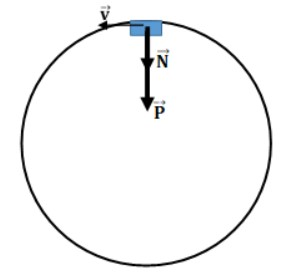
\includegraphics[scale=0.6]{../figs/VN10-2022-PH-TP0005-1.jpg}
		\end{center}
		
		Tại điểm cao nhất của vòng xiếc có các lực tác dụng lên xe là trọng lực $\vec P$ và phản lực $\vec N$ của vòng xiếc.
		
		Ta có:
		
		$$P + N = F_\text{ht} = m \dfrac{v^2}{R} \Rightarrow N = m \dfrac{v^2}{R} - P.$$
		
		Gọi $\vec N'$ là lực ép của người đi xe lên vòng xiếc, ta có:
		
		$$N' = N = \dfrac{mv^2}{R} - mg = \SI{216}{N}.$$
	}
	\item \mkstar{2}
	
	
	{Xe có khối lượng 1 tấn đi qua cầu vồng. Cầu có bán kính cong là $\SI{50}{m}$. Giả sử xe chuyển động đều với vận tốc $\SI{10}{m/s}$. Lấy $g = \SI{9,8}{m/s}^2$. Tại đỉnh cầu, tính lực nén của xe lên cầu bằng
		\begin{mcq}(4)
			\item $\SI{7200}{N}.$
			\item $\SI{5500}{N}.$
			\item $\SI{7800}{N}.$
			\item $\SI{6500}{N}.$
		\end{mcq}
	}
	
	\hideall
	{	
		\textbf{Đáp án: C.}
		
		\begin{center}
			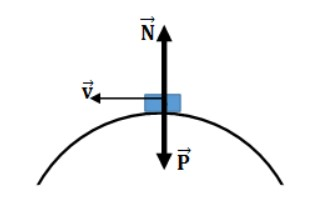
\includegraphics[scale=0.6]{../figs/VN10-2022-PH-TP0005-3.jpg}
		\end{center}
		
		Một phần trọng lực đóng vai trò là lực hướng tâm.
		
		Tại điểm cao nhất áp lực ô tô lên mặt đường là
		
		$$ N = P - F_\text{ht} = mg - \dfrac{mv^2}{R} = \SI{7800}{N}.$$
	}
	\item \mkstar{3}
	
	
	{Một máy bay thực hiện một vòng nhào lộn bán kính $\SI{400}{m}$ trong mặt phẳng thẳng đứng với vận tốc $\SI{540}{km/h}$. Lấy $g = \SI{10}{m/s}^2$. Lực do người lái có khối lượng $\SI{60}{kg}$ nén lên ghế ngồi ở điểm cao nhất và thấp nhất của vòng nhào lần lượt là
		\begin{mcq}(2)
		\item $\SI{2775}{N}; \SI{3975}{N}.$
		\item $\SI{2552}{N}; \SI{4500}{N}.$
		\item $\SI{1850}{N}; \SI{3220}{N}.$
		\item $\SI{2680}{N}; \SI{3785}{N}.$
		\end{mcq}
	}
	
	\hideall
	{	
		\textbf{Đáp án: A.}
		
		Các lực tác dụng lên người lái là trọng lực $\vec P$ và phản lực $\vec Q$ của ghế lên người.
		
		Tại vị trí cao nhất, ta có:
		
		$$P + Q = F_\text{ht} = \dfrac{mv^2}{R} \Rightarrow Q = \dfrac{mv^2}{R} - P.$$
		
		
		Gọi $\vec N$ là lực ép của người lái lên ghế tại vị trí cao nhất, ta có:
		
		$$N = Q = \dfrac{mv^2}{R} - mg = \SI{2775}{N}.$$
		
		Tại vị trí thấp nhất, ta có:
		
		$$ - P + Q = F_\text{ht} = \dfrac{mv^2}{R} \Rightarrow Q = \dfrac{mv^2}{R} + P.$$
		
		Gọi $\vec N'$ là lực ép của người lái lên ghế tại vị trí thấp nhất:
		
		$$N' = Q = \dfrac{mv^2}{R} + mg = \SI{3975}{N}.$$
	}
	\item \mkstar{2}
	
	
	{Một ô tô có khối lượng $\SI{1200}{kg}$ chuyển động đều qua một đoạn cầu vượt (coi là cung tròn) với vận tốc $\SI{36}{km/h}$. Biết bán kính cong của đoạn cầu vượt là $\SI{50}{m}$. Lấy $g = \SI{10}{m/s}^2$. Áp lực của ô tô vào mặt đường tại điểm cao nhất bằng 
		\begin{mcq}(4)
		\item $\SI{11950}{N}.$
		\item $\SI{11760}{N}.$
		\item $\SI{9600}{N}.$
		\item $\SI{14400}{N}.$
		\end{mcq}
	}
	
	\hideall
	{	
		\textbf{Đáp án: C.}
		
		\begin{center}
			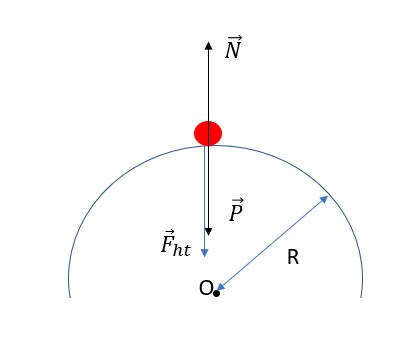
\includegraphics[scale=0.6]{../figs/VN10-2022-PH-TP0005-2.jpg}
		\end{center}
		
		Đổi $\SI{36}{km/h} = \SI{10}{m/s}.$
		
		Hợp lực của trọng lực $P$ và phản lực $N$ của mặt cầu vồng tạo ra lực hướng tâm:
		
		$$\vec P + \vec N = \vec F_\text{ht}\ (1).$$
		
		Chọn chiều dương của trục tọa độ hướng theo chiều của $P$. Chiếu biểu thức (1) lên trục đã chọn ta được:
		
		$$F_\text{ht} = P - N \Leftrightarrow m\dfrac{v^2}{R} = P - N \Rightarrow N = P - m\dfrac{v^2}{R} = mg - m\dfrac{v^2}{R} = \SI{9600}{N}.$$
	}
	\item \mkstar{2}
	
	
	{Diễn viên xiếc đi xe đạp trên vòng xiếc bán kính $\SI{6,4}{m}$. Lấy $g = \SI{10}{m/s}^2$. Để đi qua điểm cao nhất mà không rơi thì người đó phải đi với tốc độ tối thiểu bằng
		\begin{mcq}(4)
			\item $\SI{15}{m/s}.$
			\item $\SI{8}{m/s}.$
			\item $\SI{12}{m/s}.$
			\item $\SI{9,3}{m/s}.$
		\end{mcq}
	}
	
	\hideall
	{	\textbf{Đáp án: B.}
		
		Tại điểm cao nhất của vòng xiếc có các lực tác dụng lên xe là trọng lực
		
		$P$ và phản lực $Q$ của vòng xiếc.
		
		Ta có:
		
		$$P+Q = F_\text{ht} = m\dfrac{v^2}{R} \Rightarrow Q = m \dfrac{v^2}{R} - P.$$
		
		Gọi $N$ là lực ép của người đi xe lên vòng xiếc, ta có:
		
		$$N=Q = \dfrac{mv^2}{R} - mg.$$
		
		Muốn không bị rơi khỏi vòng xiếc, tức là vẫn còn lực ép lên vòng xiếc. Khi đó:
		
		$$ v \geq \sqrt{gR} = \SI{8}{m/s}.$$
	}
		\item \mkstar{2}
	
	
	{Một xe có khối lượng $m$ chuyển động trên đường cua tròn có bán kính $r = \SI{100}{m}$ với vận tốc không đổi $\SI{72}{km/h}$. Lấy $g = \SI{10}{m/s}^2$. Hệ số ma sát giữa lốp xe và mặt đường ít nhất bằng bao nhiêu để xe không trượt là
		\begin{mcq}(4)
			\item 0,35
			\item 0,26.
			\item 0,33.
			\item 0,4.
		\end{mcq}
	}
	
	\hideall
	{	
		\textbf{Đáp án: D.}
		
		Để xe không trượt thì:
		
		$$F_\text{ht} \leq F_\text{msn} \Rightarrow m \dfrac{v^2}{r} \leq \mu mg \Rightarrow \mu \geq \dfrac{v^2}{gr} = \SI{0,4}{}.$$
	}
\end{enumerate}
	\hideall
{
	\begin{center}
		\textbf{BẢNG ĐÁP ÁN}
	\end{center}
	\begin{center}
		\begin{tabular}{|m{2.8em}|m{2.8em}|m{2.8em}|m{2.8em}|m{2.8em}|m{2.8em}|m{2.8em}|m{2.8em}|m{2.8em}|m{2.8em}|}
			\hline
			1.C  & 2.C  & 3.A  & 4.C  & 5.B  & 6.D  & 7.A  & 8.B  & 9.C  & 10.B  \\
			\hline
			11.D  & 12. D  & 13.A  & 14.A  & 15.B  & 16.B  & 17.B  & 18.B  & 19.C  & 20.D  \\
			\hline
			21.C  & 22.A  & 23.C  & 24.B  & 25.D  &   &   &   &   &  \\
			\hline
		\end{tabular}
	\end{center}
}